\documentclass[11pt]{article}

% ── Layout ──
\usepackage[margin=1in]{geometry}

% ── Fonts ──
\usepackage{times}
\usepackage[T1]{fontenc}

% ── Math ──
\usepackage{amsmath,amssymb,amsfonts}

% ── Tables & Figures ──
\usepackage{booktabs,multirow}
\usepackage{graphicx,subcaption}

% ── Links ──
\usepackage[colorlinks,citecolor=blue!60!black,linkcolor=blue!60!black,urlcolor=blue!60!black]{hyperref}

% ── Units ──
\usepackage{siunitx}
\sisetup{detect-weight=true}

% ── Colors (shared with standalone TikZ figures) ──
\usepackage{xcolor}
\definecolor{ink}{HTML}{1F2937}
\definecolor{steel}{HTML}{334155}
\definecolor{cblue}{HTML}{2563EB}
\definecolor{amber}{HTML}{D97706}
\definecolor{emerald}{HTML}{059669}
\definecolor{rose}{HTML}{BE123C}
\definecolor{muted}{HTML}{64748B}
\definecolor{slatebg}{HTML}{F8FAFC}
\definecolor{gridc}{HTML}{E2E8F0}
\definecolor{gridline}{HTML}{E2E8F0}
\definecolor{mppgold}{HTML}{F59E0B}
\definecolor{flagship}{HTML}{2563EB}
\definecolor{secondary}{HTML}{D97706}
\definecolor{physgood}{HTML}{059669}
\definecolor{errbad}{HTML}{BE123C}
\definecolor{panelbg}{HTML}{F8FAFC}
\definecolor{stepblue}{HTML}{2C3E50}
\definecolor{featureteal}{HTML}{1ABC9C}
\definecolor{headpurple}{HTML}{8E44AD}
\definecolor{projred}{HTML}{C0392B}
\definecolor{splineorg}{HTML}{D35400}
\definecolor{annotgray}{HTML}{7F8C8D}
\definecolor{bgcard}{HTML}{FDFEFE}
\definecolor{accentbg}{HTML}{F7F9FB}

% ── TikZ ──
\usepackage{tikz}
\usepackage{pgfplots}
\pgfplotsset{compat=1.18}
\usetikzlibrary{arrows.meta,calc,positioning,fit,backgrounds,decorations.pathreplacing,shadows.blur}
\usepackage{standalone}

\graphicspath{{figures/}{diagnostics/}{media/}{newfigs/}{boxplots/}{NEWRESULTS/tcn_icml_20260207/figures/main_paper/}}

% ── Title ──
\title{\textbf{Physics-Informed Convolutional Surrogates for Coupled\\[4pt]
Drift-Diffusion Equations: Reconstructing Full J-V Curves\\[4pt]
of Perovskite Solar Cells}}
\author{Mehmet Ozdincer}
\date{}

\begin{document}
\maketitle

%=============================================================================
\begin{abstract}
%=============================================================================
We present a physics-constrained deep learning surrogate that reconstructs full current-voltage (J-V) curves of perovskite solar cells from 31 coupled drift-diffusion parameters spanning $>$20 orders of magnitude.
On ${\sim}15$k held-out devices the model achieves median $R^2 = 0.9975$, median MAE of $2.96$~A/m$^2$, and median $V_{oc}$ error of 0.39~mV, which is an order of magnitude below experimental measurement uncertainty, while reducing inference from ${\sim}4800$~s per COMSOL simulation to milliseconds ($>$$10^4\times$ speedup), enabling million-device screening in under one hour on a single GPU.
Physics knowledge informs every stage of the pipeline: 71 analytically derived drift-diffusion features are distilled to 5 based on the independent physical mechanisms governing J-V shape (photocurrent generation, band gap energetics, built-in field alignment, interface band alignment, recombination losses), while soft monotonicity, convexity, and curvature penalties encode qualitative PDE properties on the output.
The architecture itself is physics-motivated: bidirectional dilated convolutions provide full receptive-field coverage of the compact 8-point J-V representation, matching the thermodynamic equilibrium nature of J-V responses and their monotonically decaying spatial correlation structure, which renders self-attention redundant and consistently harmful on these short sequences.
Training completes in ${\sim}10$~min on a single NVIDIA L40S GPU.
\end{abstract}

%=============================================================================
\section{Introduction}
\label{sec:introduction}
%=============================================================================

Perovskite solar cells now exceed 26\% PCE in single-junction configurations~\cite{zhao2023phd}, but optimizing them requires navigating a 31-dimensional parameter space of bandgaps, mobilities, thicknesses, doping densities, recombination coefficients, and contact work functions, whose interactions are governed by coupled nonlinear drift-diffusion physics.

The standard computational approach is coupled Poisson--drift-diffusion simulation via COMSOL finite-element methods (FEM), which faithfully resolves the transport physics but costs ${\sim}4800$~s per device ($\sim$ 160 years for a typical 10$^6$ device campaign), making its use for high-throughput and manufacturing-side research at labs like SERIS infeasible.

Zhao et al.~\cite{zhao2025ae} achieved $>$$10^3\times$ speedup for \emph{scalar} metrics ($V_{oc}$, FF, PCE) via neural network surrogates.
However, these metrics do not capture device characteristics that may be derived from full curves including: S-shaped kinks from interface barriers, fill-factor degradation modes, and the drift-to-recombination transition at the maximum power point.
Two devices with identical PCE can have qualitatively different J-V curves and correspondingly different operational characteristics.

We address this gap with the following contributions:
\begin{enumerate}
    \item \textbf{First full J-V curve surrogate from coupled drift-diffusion parameters} (\S\ref{sec:results}): median $R^2 = 0.9975$, median $V_{oc}$ error of 0.39~mV (below experimental measurement uncertainty), and $>$$10^4\times$ speedup over COMSOL FEM, which reduces a $10^6$-device screening campaign from ${\sim}160$~years to under one hour on a single GPU.

    \item \textbf{Physics-driven feature engineering} (\S\ref{sec:physics_features}--\ref{sec:feature_selection}): we derive 71 analytical drift-diffusion features and select 5 based on physical reasoning about the independent mechanisms governing J-V shape, photocurrent generation, band gap energetics, built-in field alignment, interface band alignment, and recombination losses, with multicollinearity analysis (175 pairs at $|r|>0.85$) supporting the selection.

    \item \textbf{Domain-matched architecture design} (\S\ref{sec:architecture}--\ref{sec:ablation}): bidirectional dilated convolutions provide full receptive-field coverage of the 8-point J-V sequence, matching the physical structure of thermodynamic equilibrium responses where spatial correlations decay monotonically with voltage separation, which rendered self-attention redundant and consistently harmful.

    \item \textbf{Physics-native representation pipeline} (\S\ref{sec:preprocessing}--\ref{sec:loss}): a co-designed pipeline where each component exploits specific physical structure of J-V curves---monotone PCHIP compression ($45 \to 8$ points) simultaneously reduces output dimensionality and encodes a shape prior, learnable Gaussian RBF voltage embeddings give the convolutional backbone a continuous voltage coordinate matching the non-uniform grid physics, $J_{sc}$-normalization decouples current magnitude from curve shape, and soft monotonicity/convexity/curvature penalties encode qualitative PDE properties without requiring PDE evaluation during training.
\end{enumerate}

%=============================================================================
\section{Results}
\label{sec:results}
%=============================================================================

Figure~\ref{fig:random_samples} displays J-V reconstructions for randomly sampled test devices spanning the full performance range.
The model's 8-point PCHIP representation, interpolated back to a dense voltage grid via Fritsch--Carlson monotone cubic Hermite interpolation~\cite{fritsch1980monotone}, faithfully captures both the flat photocurrent plateau at low voltages and the sharp sigmoidal transition at the knee/MPP region.
The vast majority of devices achieve $R^2 > 0.99$; the rare low-$R^2$ cases correspond to pathological device configurations discussed in \S\ref{sec:failure_analysis}.

\begin{figure}[t]
    \centering
    \includegraphics[width=0.95\textwidth]{test_plots_random_samples.png}
    \caption{\textbf{Random test-set reconstructions} ($R^2 = 0.58$--$0.999$). Blue circles: 8 PCHIP query points predicted by the dilated conv model; dashed: PCHIP reconstruction; solid grey: COMSOL finite-element reference. The model captures flat-band plateaus, sharp knees, and the approach to $V_{oc}$ across devices with widely varying material parameters. The rare low-$R^2$ cases (bottom row) correspond to S-shaped or barrier-dominated devices where physics constraints \emph{correctly refuse} unphysical fits (\S\ref{sec:failure_analysis}).}
    \label{fig:random_samples}
\end{figure}

\subsection{Primary Performance}
\label{sec:primary_performance}

Table~\ref{tab:primary_results} reports performance of the primary model (bidirectional dilated conv, batch size 512, with physics features) on the held-out test set, averaged over 3 random seeds.

\begin{table}[t]
\centering
\caption{Test-set performance (${\sim}15$k devices), averaged over 3 seeds ($\pm$ seed-to-seed std). The mean--median gap in $R^2$ reflects a long left tail from pathological devices (\S\ref{sec:failure_analysis}), not systematic bias.}
\label{tab:primary_results}
\begin{tabular}{@{}lrr@{}}
\toprule
\textbf{Metric} & \textbf{Mean} & \textbf{Median} \\
\midrule
$R^2$ (per-curve, $\Delta V$-weighted) & $0.9858 \pm 0.0009$ & $\mathbf{0.9975 \pm 0.0004}$ \\
MAE (A/m$^2$) & $4.75 \pm 0.26$ & $2.96 \pm 0.34$ \\
RMSE (A/m$^2$) & $6.66 \pm 0.26$ & $4.27 \pm 0.34$ \\
$|V_{oc}$ error$|$ (V) & $0.0056 \pm 0.0058$ & $\mathbf{0.00039 \pm 0.00016}$ \\
$|I_{sc}$ error$|$ (A/m$^2$) & $0.59 \pm 0.53$ & $0.36 \pm 0.62$ \\
\bottomrule
\end{tabular}
\end{table}

\paragraph{Physical significance.}
The median MAE of 2.96~A/m$^2$ corresponds to $<$0.5\% of a typical $J_{sc} \approx 200$~A/m$^2$, meaning the model faithfully resolves both the flat-band photocurrent magnitude and the sharp transition at MPP where most power extraction occurs.
The $I_{sc}$ median error of 0.36~A/m$^2$ (with seed-to-seed variability of $\pm$0.62) confirms that the flat-band region ($V \ll V_{mpp}$) is trivially learned, consistent with the physics, since $J(V \!\approx\! 0) \approx J_{sc}$ is determined primarily by photogeneration and collection efficiency, which are well-captured by the input features.

The median $V_{oc}$ error of 0.39~mV is an order of magnitude below typical experimental measurement uncertainty ($\pm$5~mV for perovskite devices with hysteresis), meaning the model's voltage-axis localization of the open-circuit point is more precise than what current fabrication and measurement technology can resolve.
This sub-millivolt precision in $V_{oc}$ reconstruction is important because $V_{oc}$ determines the upper voltage bound of the J-V curve, and errors in $V_{oc}$ propagate into the reconstructed current values throughout the knee region where $dJ/dV$ is large.

\paragraph{The mean--median gap.}
The gap between mean $R^2 = 0.986$ and median $R^2 = 0.998$ indicates that fewer than 1\% of devices account for the majority of aggregate error.
This asymmetry is by design: the physics constraints \emph{correctly refuse} to fit S-shaped or concave-up curves that violate the monotone-sigmoid assumption (\S\ref{sec:failure_analysis}).
A model that achieved higher mean $R^2$ by fitting these pathological devices would necessarily sacrifice physical plausibility on the remaining 99\%.

\paragraph{Computational performance.}
Total wall time: ${\sim}10$~min (preprocessing 24~s, training ${\sim}9.5$~min, inference ${\sim}10$~s on ${\sim}15$k test samples).
Training throughput: ${\sim}12.7$k samples/s (batch size 512); inference throughput: ${\sim}1.4$k samples/s.
This represents $>$$10^4\times$ speedup over COMSOL FEM per device, enabling a $10^6$-device Latin Hypercube screening sweep in $<$1~hour.
\subsection{Architecture Design Rationale}
\label{sec:ablation}

Each architectural decision is motivated by the physics of J-V curves and validated empirically (full 30-run ablation in Appendix~\ref{app:ablation}).

\paragraph{Spatial mixing: inter-voltage coupling is physically required.}
J-V curves are smooth, monotone responses governed by coupled transport equations, which state that the current at any voltage depends on the carrier distribution across the \emph{entire} device.
A pointwise ($1{\times}1$) baseline that predicts each voltage independently achieves only $R^2_{med} = 0.989$, compared to $0.997$ for the dilated conv, confirming that the architecture must exchange information across voltage points to capture the interdependence encoded in the drift-diffusion equations.

\paragraph{Bidirectional context: equilibrium, not causality.}
J-V curves describe \emph{thermodynamic equilibrium} responses, not temporal sequences: at any applied voltage, the current depends on the full band diagram ($V_{bi} - V$ across all layers), recombination at both interfaces, and extraction at both contacts.
Causal (unidirectional) masking discards this bidirectional physical dependence, and indeed the causal TCN shows $3.9\times$ higher $V_{oc}$ error variance than the bidirectional conv ($1.51 \pm 1.68$~mV vs.\ $0.39 \pm 0.16$~mV), with instability concentrated near $V_{oc}$ where the causal architecture lacks access to high-voltage context.

\paragraph{Dilated convolutions: full receptive field without attention.}
Block~3's dilation $d{=}2$ with kernel $k{=}5$ yields a single-layer receptive field of 9 positions, already exceeding the 8-point sequence length.
This architectural property has a direct physical consequence: because every output position already has bidirectional context over all input positions, the $\mathcal{O}(n^2)$ pairwise interactions of self-attention are redundant.
Empirically, adding 4-head attention degrades median $R^2$ from ${\sim}0.997$ to ${\sim}0.991$ across both Conv and TCN backbones (Appendix~\ref{app:ablation}, Figure~\ref{fig:attention_impact}).
The underlying reason is structural: J-V spatial correlations decay monotonically with voltage separation, matching convolution's local inductive bias, while attention treats all voltage pairs uniformly and amplifies noise from weakly coupled points.

\paragraph{Batch size 512: gradient noise meets the loss landscape.}
Increasing batch size from 128 to 512 yields the largest single-factor improvement ($R^2_{med}$: $0.9964 \to 0.9975$; MAE: $3.74 \to 2.96$~A/m$^2$) while halving training time to ${\sim}10$~min.
The physics-constrained loss (Eq.~\ref{eq:loss}) combines five terms with different gradient scales; larger batches reduce per-term gradient variance, enabling more stable optimization of the multi-objective landscape.

\subsection{Failure Mode Analysis}
\label{sec:failure_analysis}

The left tail of the $R^2$ distribution ($R^2_{mean} = 0.986$ vs.\ $R^2_{med} = 0.998$, affecting $<$1\% of devices) arises from three physically distinct failure modes, each traceable to a specific violation of the assumptions encoded in the model's architecture and loss:

\begin{enumerate}
    \item \textbf{S-shaped / concave-up curves}: Large interface band offsets ($|\Delta E_v^{HP}|$ or $|\Delta E_c^{PE}| \gg k_BT$) produce barrier-dominated transport where the J-V curve exhibits a local current \emph{increase} with voltage (the ``S-kink''), violating the monotone-sigmoid assumption inherent in the PCHIP representation.
    Physically, S-kinks arise when extraction barriers at one interface force carriers to accumulate, creating a voltage-dependent barrier height that produces non-monotone current response.
    The monotonicity constraint \emph{correctly refuses} to fit these curves: the model produces a smooth sigmoid approximation rather than an unphysical reconstruction.
    This is a deliberate trade-off: capturing S-shaped behavior would require abandoning the monotone PCHIP representation and significantly increasing output dimensionality, at the cost of less constrained predictions for the 99\%+ well-behaved devices.
    Notably, this failure mode correlates strongly with $|\Delta E_v^{HP}| \gg k_BT$ and large $|E_g^{offset}|$, both of which are among the selected physics features, meaning the model has the information to \emph{detect} these devices even though it cannot faithfully \emph{reconstruct} them.

    \item \textbf{Mislocated knee}: When $V_{oc}$ falls far from the training-set center (typically $V_{oc} < 0.5$~V or $V_{oc} > 1.2$~V), the sigmoid transition occurs outside the dense query-point region, and the 8-point budget lacks resolution where it is most needed.
    This is a consequence of the fixed query-point grid: the points are concentrated near the \emph{typical} MPP voltage, but extreme-$V_{oc}$ devices have their steepest curvature elsewhere.
    Adaptive query-point placement conditioned on predicted $V_{oc}$ would address this failure mode while preserving the compact 8-point representation.

    \item \textbf{Extreme series resistance}: $R_s^{total} > 10^3$~$\Omega\!\cdot\!\text{cm}^2$ produces nearly linear J-V curves ($J(V) \approx J_{sc} - V/R_s$) that are qualitatively unlike the sigmoid majority.
    The convexity and curvature penalties are designed for sigmoidal shapes and actively resist linear reconstructions.
    These devices have $\text{FF} \ll 0.5$ and represent impractical configurations that would never be fabricated.
    Consistent with this, $R_s^{total}$ achieved $|r| < 0.001$ with target variables during feature selection (\S\ref{sec:feature_selection}), confirming that resistive effects are negligible for the vast majority of the parameter space.
\end{enumerate}

In all three cases, the failure mode is \emph{physically interpretable} and corresponds to devices outside the intended operating regime.
The physics features themselves enable a lightweight anomaly detector: a simple threshold on $|E_g^{offset}|$, $|\Delta E_v^{HP}|$, and $R_s^{total}$ can flag pathological devices at negligible computational cost before running inference, providing a built-in reliability indicator.

Figures~\ref{fig:best_r2} and~\ref{fig:worst_r2} contrast the best and worst reconstructions, making the failure modes visually concrete.

\begin{figure}[t]
    \centering
    \includegraphics[width=0.95\textwidth]{test_plots_best_r2_samples.png}
    \caption{\textbf{Best $R^2$ reconstructions} ($\approx 1.000$): near-perfect reconstruction for well-behaved sigmoid curves with clear knee regions. These devices have favorable energetic alignment ($E_g^{offset} \approx 0$), moderate barrier heights, and high $J_{max}$, placing them squarely within the model's physics-constrained operating regime.}
    \label{fig:best_r2}
\end{figure}

\begin{figure}[t]
    \centering
    \includegraphics[width=0.95\textwidth]{test_plots_worst_r2_samples.png}
    \caption{\textbf{Worst $R^2$ reconstructions} ($< 0$): S-shaped kinks (barrier-dominated transport), concave-up curves, and extreme-resistance configurations. In each case, the physics constraints \emph{correctly prevent} unphysical fits, producing smooth sigmoid approximations instead. These devices have large $|E_g^{offset}|$, extreme $|\chi_P^e|$ values, or $|\Delta E_v^{HP}| \gg k_BT$, violating the monotone-sigmoid assumption inherent in the PCHIP representation.}
    \label{fig:worst_r2}
\end{figure}

\section{Background: Drift-Diffusion Model}
\label{sec:comsol}

The ground-truth J-V curves are generated by a coupled Poisson--drift-diffusion simulator~\cite{zhao2023phd,zhao2025ae} modeling a planar p-i-n perovskite stack: Glass / Front-contact / HTL / Perovskite absorber / ETL / Back-contact.
Optical absorption follows a vectorized transfer-matrix formulation (Appendix~\ref{app:optical}) yielding the spatially averaged photogeneration rate $G_{avg} = l_P^{-1}\int_0^{l_P} G(x)\,dx$, which enters as one of the 31 inputs.

The electronic transport is governed by three coupled PDEs:
\begin{align}
\nabla \cdot (\varepsilon \nabla \psi) &= -q(p - n + N_D^+ - N_A^-) \label{eq:poisson} \\
\frac{\partial n}{\partial t} &= \frac{1}{q} \nabla \cdot \mathbf{J}_n - R + G \label{eq:electron} \\
\frac{\partial p}{\partial t} &= -\frac{1}{q} \nabla \cdot \mathbf{J}_p - R + G \label{eq:hole}
\end{align}
where the current densities follow drift-diffusion:
\begin{equation}
\mathbf{J}_n = qn\mu_n\mathbf{E} + qD_n\nabla n, \qquad
\mathbf{J}_p = qp\mu_p\mathbf{E} - qD_p\nabla p
\label{eq:drift_diffusion}
\end{equation}
with diffusion coefficients related to mobilities through the Einstein relation $D = \mu k_B T / q$.

Recombination combines radiative, Shockley-Read-Hall (SRH), Auger, and interface terms:
\begin{align}
R_{rad} &= B_{rad}(np - n_i^2) \label{eq:recomb_rad} \\
R_{SRH} &= \frac{np - n_i^2}{\tau_h(n{+}n_1) + \tau_e(p{+}p_1)} \label{eq:recomb_srh} \\
R_{Aug} &= (A_e n + A_h p)(np - n_i^2) \label{eq:recomb_aug}
\end{align}
with intrinsic carrier concentration $n_i = \sqrt{N_c N_v}\exp(-E_g/2k_BT)$, built-in voltage $V_{bi} = W_{anode} - W_{cathode}$, and interface recombination velocity $j_s = v_s \Delta c$.

The system is solved in COMSOL at each applied voltage $V$ to generate the $J(V)$ curve.
The 31 input parameters (Table~\ref{tab:31params}) span $>$20 orders of magnitude, from carrier mobilities (${\sim}10^{-4}$--$10^{2}$~cm$^2$/Vs) to doping densities (${\sim}10^{17}$--$10^{21}$~cm$^{-3}$) to recombination coefficients (${\sim}10^{-12}$--$10^{-6}$~cm$^3$/s), necessitating careful preprocessing (\S\ref{sec:preprocessing}).

\begin{table}[t]
\centering
\caption{The 31 COMSOL parameters grouped by physical origin. Parameters span $>$20 orders of magnitude, with six per-layer quantities (band edges, mobilities), three layer thicknesses, and global recombination/generation parameters.}
\label{tab:31params}
\begin{tabular}{@{}lcp{8cm}@{}}
\toprule
\textbf{Group} & $n$ & \textbf{Parameters} \\
\midrule
Band edges & 6 & $\chi_{e,h}$ for ETL, perovskite, HTL (eV) \\
Mobilities & 6 & $\mu_{n,p}$ per layer (cm$^2$/Vs) \\
Thicknesses & 3 & $l_H, l_P, l_E$ (nm) \\
SRH lifetimes & 2 & $\tau_e, \tau_h$ (s) \\
Density of states & 4 & $N_{c,v}$ for perovskite and ETL (cm$^{-3}$) \\
Recombination & 4 & $v_{IV,V}$ (cm/s), $B_{rad}$ (cm$^3$/s), $C_{Aug}$ (cm$^6$/s) \\
Permittivities & 3 & $\varepsilon$ per layer (relative) \\
Contacts & 2 & $W_{anode}$, $W_{cathode}$ (eV) \\
Generation & 1 & $G_{avg}$ (cm$^{-3}$s$^{-1}$) \\
\bottomrule
\end{tabular}
\end{table}

\section{Two-Stage Surrogate Pipeline}
\label{sec:scalar_pipeline}

The framework operates as a modular two-stage pipeline (Figure~\ref{fig:pipeline}):

\paragraph{Stage~1: Scalar prediction (Zhao et al.~\cite{zhao2025ae}).}
Three-layer ANNs with Bayesian regularization, trained on 100k LHS samples, predict scalar device metrics from the 31 raw parameters:
\begin{equation}
\mathbf{x} \in \mathbb{R}^{31} \xrightarrow[\text{Zhao et al.}]{\text{3-layer ANN}} \{V_{oc}^{pred}, V_{mpp}^{pred}, J_{sc}^{pred}\}
\label{eq:scalar_stage}
\end{equation}
with MSE $< 3.1 \times 10^{-4}$ for $V_{oc}$, validated against 9 fabricated devices spanning $E_g \in \{1.56, 1.63\}$~eV (calibration MSE $8.2 \times 10^{-8}$--$1.8 \times 10^{-4}$)~\cite{zhao2025ae}.

\paragraph{Stage~2: Curve reconstruction (this work).}
Pre-computed scalar predictions condition the curve model alongside 31 scaled parameters and $m$ selected physics features:
\begin{equation}
\mathbf{x}_{in} = [\,\underbrace{\mathbf{x}^{sc}}_{31}\;;\;\underbrace{V_{oc}^{pred},\, V_{mpp}^{pred}}_{\text{Stage 1}}\;;\;\underbrace{\boldsymbol{\phi}(\mathbf{x})}_{m}\,]
\xrightarrow{f_\theta} \hat{\mathbf{J}} \in \mathbb{R}^{8}
\label{eq:curve_stage}
\end{equation}
where $m = 5$ after train-only feature selection (\S\ref{sec:feature_selection}).

This design prevents inter-stage gradient leakage, enables swapping ground-truth for predicted scalars during ablation, and allows independent training of each stage.

\begin{figure}[t]
    \centering
    \resizebox{\textwidth}{!}{\input{figures/pipeline.tex}}
    \caption{\textbf{Two-stage surrogate pipeline.}
    Stage~1: ANNs~\cite{zhao2025ae} predict scalar metrics from 31 parameters.
    Stage~2: dilated conv model consumes scaled parameters, Stage~1 scalars, and $m{=}5$ physics features to produce 8-point J-V curves under physics-constrained loss.}
    \label{fig:pipeline}
\end{figure}

\section{Related Work}
\label{sec:litreview}

\paragraph{ML surrogates for perovskites.}
Prior machine learning surrogates for perovskite solar cells predict scalar properties: band gap from composition~\cite{feng2024bandgap}, formability classification~\cite{talapatra2021formability}, lattice constants~\cite{zhang2020lattice}, and device-level metrics (PCE, FF)~\cite{hu2022ml,oboh2024nn}.
None predict full J-V curves from material parameters.

\paragraph{J-V curve prediction.}
Two concurrent works address J-V reconstruction for perovskite devices (Table~\ref{tab:comparison}).
Toprak~\cite{toprak2025jv} mapped irradiance and voltage $(G, V)$ to current density $J$ for a \emph{single fixed device geometry} (2 input dimensions, $R^2 = 0.994$, 8k training samples).
Zbinden et al.~\cite{zbinden2026ae} used conditional variational autoencoders for forward and inverse J-V modeling from 6 fabrication parameters ($R^2 = 0.996$, 50k training samples, validated on 4 fabricated devices).
Our work generalizes across 31 coupled drift-diffusion dimensions with ${\sim}150$k training samples and explicit physics constraints, and contributes the architectural finding that bidirectional convolutions outperform attention-based and point-wise architectures on short physics-governed sequences.

\begin{table}[t]
\centering
\caption{Comparison with concurrent J-V curve reconstruction approaches. Our method operates in the highest-dimensional parameter space with the largest training set and strongest physics constraints.}
\label{tab:comparison}
\begin{tabular}{@{}lcccc@{}}
\toprule
& \textbf{Toprak}~\cite{toprak2025jv} & \textbf{Zbinden}~\cite{zbinden2026ae} & \textbf{Ours} \\
\midrule
Input dimensions & 2 & 6 & 31 + $m$ \\
Architecture & MLP & Conditional AE & Dilated Conv \\
Training data & 8k & 50k & 150k \\
Best $R^2$ & 0.994 & 0.996 & \textbf{0.998} \\
Physics constraints & -- & Latent regularization & Mono+conv+curv \\
Inverse design & No & Encoder-based & Gradient-based \\
Experimental validation & No & 4 devices & Via~\cite{zhao2025ae}: 9 devices \\
\bottomrule
\end{tabular}
\end{table}

\paragraph{Physics-informed neural networks (PINNs).}
Classical PINNs embed PDE residuals as loss terms, requiring PDE evaluation during training.
Our approach instead uses physics to \emph{inform inputs} (71 derived features) and \emph{constrain outputs} (monotonicity, convexity, curvature), avoiding PDE evaluation entirely.
This is closer to the ``physics-informed feature engineering'' paradigm than to residual-based PINNs.


\section{Method}
\label{sec:method}

\subsection{Problem Formulation}

Given device parameters $\mathbf{x} \in \mathbb{R}^{31}$ and upstream scalar predictions $\{V_{oc}^{pred}, V_{mpp}^{pred}\}$, predict a compact J-V representation:
\begin{equation}
\hat{\mathbf{J}} = f_\theta(\mathbf{x}_{in}; \mathbf{V}_{query}) \in \mathbb{R}^8
\end{equation}
where $\mathbf{V}_{query}$ are 8 voltage query points concentrated near the MPP.
Convention: positive photocurrent ($J > 0$ for $V < V_{oc}$).
The full 45-point J-V curve is recovered via PCHIP interpolation from the 8 predicted points.

\subsection{Data}
\label{sec:data}

Two LHS campaigns generate the ground-truth dataset:
\begin{itemize}
    \item \textbf{Campaign 1}: 100k samples $\to$ usable subset after COMSOL convergence filtering
    \item \textbf{Campaign 2}: 300k samples $\to$ usable subset after filtering
    \item \textbf{Combined}: ${\sim}$150k devices after convergence and quality filtering, split 80/10/10 train/val/test (120k/15k/15k)
\end{itemize}

Filtering removes only devices where COMSOL failed to converge or produced grossly unphysical curves (e.g., negative $J_{sc}$, $V_{oc} < 0$); no curvature-based or performance-based filtering is applied, preserving the full LHS distribution including pathological devices.

The voltage grid is \textbf{non-uniform} (Figure~\ref{fig:voltage_grid}), with resolution concentrated where device-performance sensitivity is highest:
\begin{itemize}
    \item \textbf{Low voltage} ($0 \leq V \leq 0.4$~V): 5 coarse points, $\Delta V = 0.1$~V
    \item \textbf{Knee/MPP region} ($0.425 \leq V \leq 1.4$~V): 40 dense points, $\Delta V = 0.025$~V
    \item \textbf{Total}: $N_V = 45$ points
\end{itemize}

This design reflects the physics: the flat-band region ($V \ll V_{mpp}$) has $J \approx J_{sc}$ with near-zero curvature, while the knee region contains the MPP, the drift-to-recombination transition, and the approach to $V_{oc}$, all critical for fill-factor evaluation and device optimization.
The non-uniform spacing necessitates $\Delta V$-weighted evaluation metrics (\S\ref{sec:metrics}).

\begin{figure}[t]
    \centering
    \resizebox{\textwidth}{!}{
% Figure 4: Non-Uniform Voltage Grid + ΔV-Weighted Metric
% Compile: pdflatex fig4_voltage_grid.tex
\documentclass[border=4pt]{standalone}
\usepackage{tikz}
\usepackage{amsmath,amssymb}
\usepackage{pgfplots}
\pgfplotsset{compat=1.18}
\usetikzlibrary{arrows.meta,calc,decorations.pathreplacing}

% ── ICML Global Colour System ──
\definecolor{ink}{HTML}{1F2937}
\definecolor{flagship}{HTML}{2563EB}
\definecolor{secondary}{HTML}{D97706}
\definecolor{physgood}{HTML}{059669}
\definecolor{errbad}{HTML}{BE123C}
\definecolor{muted}{HTML}{64748B}
\definecolor{panelbg}{HTML}{F8FAFC}
\definecolor{gridline}{HTML}{E2E8F0}
\definecolor{mppgold}{HTML}{F59E0B}

\begin{document}
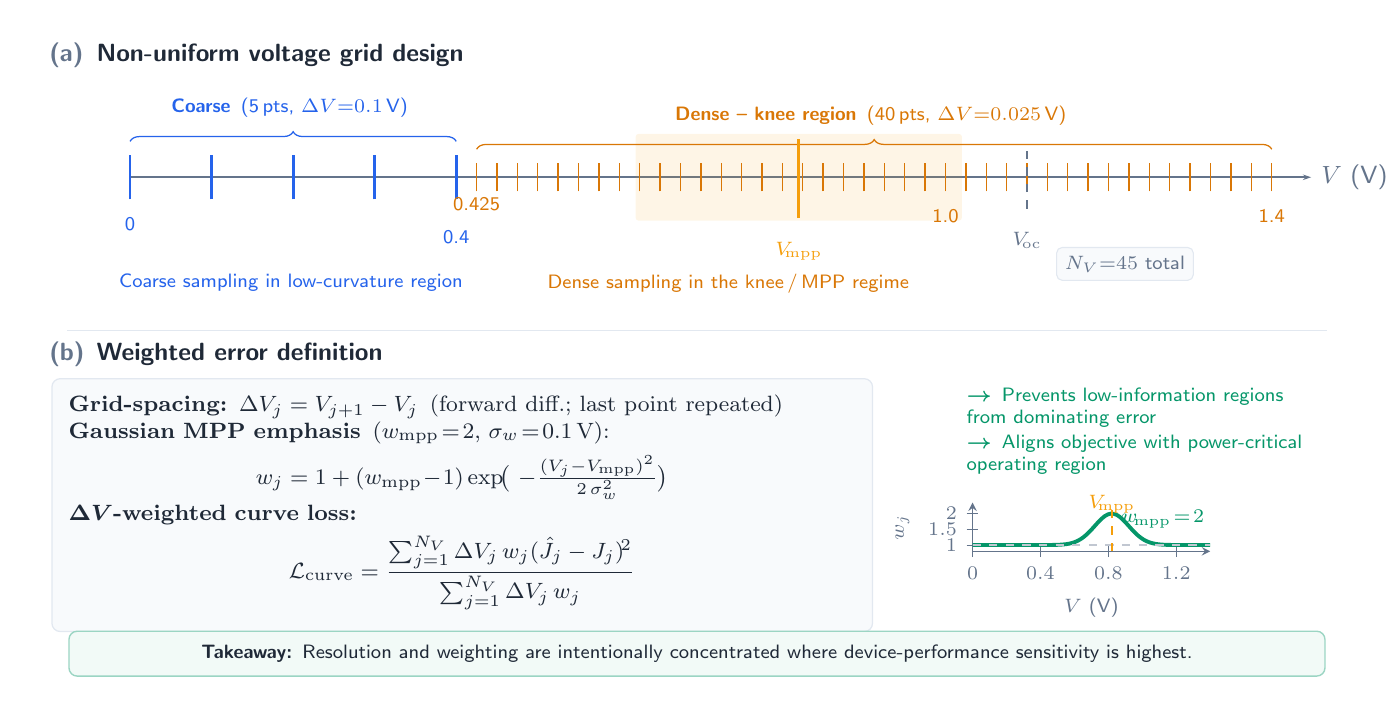
\begin{tikzpicture}[every node/.style={font=\sffamily,text=ink}]

% ── Canvas: 17.0 cm × 8.2 cm ──
\useasboundingbox (0,0) rectangle (17,8.2);

% ════════════════════════════════════════════════
%  PANEL (a)  -  Non-uniform voltage grid design
% ════════════════════════════════════════════════
\node[font=\sffamily\small\bfseries,text=muted,anchor=west]
  at (0.15,7.85) {(a)};
\node[font=\sffamily\small\bfseries,anchor=west]
  at (0.75,7.85) {Non-uniform voltage grid design};

% ── Axis geometry ──
\pgfmathsetmacro{\axL}{1.3}           % left end (cm)
\pgfmathsetmacro{\axR}{15.8}          % right end (cm)
\pgfmathsetmacro{\axY}{6.30}          % axis y-position
\pgfmathsetmacro{\vs}{(\axR-\axL)/1.4}% cm per volt

% Horizontal voltage axis
\draw[-{Stealth[length=3pt,width=2pt]},line width=0.7pt,muted]
  (\axL,\axY) -- (\axR+0.5,\axY)
  node[right,font=\sffamily\small,text=muted]{$V$ (V)};

% ── MPP highlight zone (light alpha fill) ──
\fill[mppgold,opacity=0.10,rounded corners=1pt]
  ({\axL+0.62*\vs},{\axY-0.55})
  rectangle ({\axL+1.02*\vs},{\axY+0.55});

% ── Coarse ticks: 0-0.4 V, ΔV = 0.1 V, 5 pts ──
\foreach \v in {0.0,0.1,0.2,0.3,0.4}{
  \pgfmathsetmacro{\xp}{\axL+\v*\vs}
  \draw[flagship,line width=1.0pt]
    (\xp,{\axY-0.28}) -- (\xp,{\axY+0.28});
}
\node[below=3pt,font=\sffamily\scriptsize,text=flagship]
  at (\axL,{\axY-0.28}) {0};
\node[below=8pt,font=\sffamily\scriptsize,text=flagship]
  at ({\axL+0.4*\vs},{\axY-0.28}) {0.4};

% Coarse brace - single-line spec
\draw[decorate,decoration={brace,amplitude=3.5pt,raise=5pt},
  line width=0.45pt,flagship]
  (\axL,{\axY+0.28}) -- ({\axL+0.4*\vs},{\axY+0.28})
  node[midway,above=10pt,font=\sffamily\scriptsize,text=flagship,
       align=center]{
    \textbf{Coarse}\enspace(5\,pts, $\Delta V{=}0.1$\,V)
  };

% ── Dense ticks: 0.425-1.4 V, ΔV = 0.025 V, 40 pts ──
\foreach \i in {0,1,...,39}{
  \pgfmathsetmacro{\v}{0.425+\i*0.025}
  \pgfmathsetmacro{\xp}{\axL+\v*\vs}
  \draw[secondary,line width=0.5pt]
    (\xp,{\axY-0.18}) -- (\xp,{\axY+0.18});
}
\node[below=1pt,font=\sffamily\scriptsize,text=secondary]
  at ({\axL+0.425*\vs},{\axY-0.10}) {0.425};
\node[below=3pt,font=\sffamily\scriptsize,text=secondary]
  at ({\axL+1.0*\vs},{\axY-0.18}) {1.0};
\node[below=3pt,font=\sffamily\scriptsize,text=secondary]
  at ({\axL+1.4*\vs},{\axY-0.18}) {1.4};

% Dense brace - single-line spec
\draw[decorate,decoration={brace,amplitude=3.5pt,raise=5pt},
  line width=0.45pt,secondary]
  ({\axL+0.425*\vs},{\axY+0.18}) -- ({\axL+1.4*\vs},{\axY+0.18})
  node[midway,above=10pt,font=\sffamily\scriptsize,text=secondary,
       align=center]{
    \textbf{Dense -- knee region}\enspace
    (40\,pts, $\Delta V{=}0.025$\,V)
  };

% ── Vmpp marker (label below to avoid brace overlap) ──
\pgfmathsetmacro{\xmpp}{\axL+0.82*\vs}
\draw[mppgold,line width=1.2pt]
  (\xmpp,{\axY-0.52}) -- (\xmpp,{\axY+0.48});
\node[below=5pt,font=\sffamily\scriptsize\bfseries,text=mppgold]
  at (\xmpp,{\axY-0.52}) {$V_{\!\mathrm{mpp}}$};

% ── Voc marker ──
\pgfmathsetmacro{\xvoc}{\axL+1.1*\vs}
\draw[muted,line width=0.6pt,dashed]
  (\xvoc,{\axY-0.40}) -- (\xvoc,{\axY+0.38});
\node[below=5pt,font=\sffamily\scriptsize,text=muted]
  at (\xvoc,{\axY-0.40}) {$V_{\!\mathrm{oc}}$};

% ── Required annotation callouts (colour-coded, below axis) ──
\node[font=\sffamily\scriptsize,text=flagship,anchor=north east]
  at ({\axL+0.42*\vs},{\axY-1.10})
  {Coarse sampling in low-curvature region};
\node[font=\sffamily\scriptsize,text=secondary,anchor=north west]
  at ({\axL+0.50*\vs},{\axY-1.10})
  {Dense sampling in the knee\,/\,MPP regime};

% Total-point badge
\node[draw=gridline,fill=panelbg,rounded corners=2pt,
  font=\sffamily\scriptsize,text=muted,inner sep=3pt]
  at ({\axL+1.22*\vs},{\axY-1.10})
  {$N_V{=}45$ total};

% ── Subtle panel separator ──
\draw[gridline,line width=0.35pt] (0.5,4.35) -- (16.5,4.35);

% ════════════════════════════════════════════════
%  PANEL (b)  -  Weighted error definition
% ════════════════════════════════════════════════
\node[font=\sffamily\small\bfseries,text=muted,anchor=west]
  at (0.15,4.05) {(b)};
\node[font=\sffamily\small\bfseries,anchor=west]
  at (0.75,4.05) {Weighted error definition};

% ── Equation card (compact, left column) ──
\node[
  draw=gridline,fill=panelbg,rounded corners=3pt,
  line width=0.45pt,
  text width=10.0cm,align=left,
  font=\footnotesize,text=ink,
  inner sep=6pt,anchor=north west,
] (eqnbox) at (0.3,3.75) {%
  \begingroup
  \abovedisplayskip=3pt
  \belowdisplayskip=1pt
  \abovedisplayshortskip=2pt
  \belowdisplayshortskip=1pt
  %
  \textbf{Grid-spacing:}
  $\Delta V_j = V_{j+1} - V_j$%
  \enspace(forward diff.; last point repeated)%
  \par%
  \textbf{Gaussian MPP emphasis}%
  \enspace($w_{\mathrm{mpp}}\!=\!2$, $\sigma_w\!=\!0.1$\,V):%
  \[
    w_j =  1 + (w_{\mathrm{mpp}}\!-\!1)
    \exp\!\bigl(\
    -\tfrac{(V_j - V_{\mathrm{mpp}})^{2}}{2\,\sigma_w^{2}}
    \bigr)
  \]%
  \textbf{$\boldsymbol{\Delta V}$-weighted curve loss:}%
  \[
    \mathcal{L}_{\mathrm{curve}}
    = 
    \frac{%
      \textstyle\sum_{j=1}^{N_V}
      \Delta V_j \, w_j 
      (\hat{J}_j - J_j)^{\!2}
    }{%
      \textstyle\sum_{j=1}^{N_V}
      \Delta V_j \, w_j
    }
  \]%
  \endgroup
};

% ── Right column: annotation callouts ──
\node[font=\sffamily\scriptsize,text=physgood,
  anchor=north west,text width=4.4cm,align=left]
  at (11.8,3.75) {%
    $\boldsymbol{\rightarrow}$\enspace
    Prevents low-information regions
    from dominating error%
  };
\node[font=\sffamily\scriptsize,text=physgood,
  anchor=north west,text width=4.4cm,align=left]
  at (11.8,3.15) {%
    $\boldsymbol{\rightarrow}$\enspace
    Aligns objective with
    power-critical operating region%
  };

% ── Right column: mini Gaussian-weight plot ──
\begin{scope}[shift={(12.0,1.55)}]
  \begin{axis}[
    width=4.6cm,height=2.2cm,
    at={(0,0)},anchor=south west,
    xlabel={$V$ (V)},ylabel={$w_j$},
    xlabel style={font=\sffamily\scriptsize,text=muted},
    ylabel style={font=\sffamily\scriptsize,text=muted},
    tick label style={font=\sffamily\scriptsize,text=muted},
    xmin=0,xmax=1.4,ymin=0.8,ymax=2.35,
    axis lines=left,
    axis line style={line width=0.35pt,color=muted},
    every tick/.style={muted,line width=0.25pt},
    xtick={0,0.4,0.8,1.2},
    ytick={1.0,1.5,2.0},
    grid=none,clip=false,
  ]
    \addplot[physgood,line width=1.4pt,smooth,samples=80,domain=0:1.4]
      {1.0 + 1.0*exp(-((x-0.82)^2)/(2*0.1^2))};
    \addplot[muted!40,line width=0.4pt,dashed,domain=0:1.4] {1.0};
    \draw[mppgold,line width=0.6pt,dashed]
      (axis cs:0.82,0.8) -- (axis cs:0.82,2.15);
    \node[font=\sffamily\scriptsize,text=mppgold]
      at (axis cs:0.82,2.30) {$V_{\!\mathrm{mpp}}$};
    \node[font=\sffamily\scriptsize,text=physgood]
      at (axis cs:1.12,1.82) {$w_{\!\mathrm{mpp}}\!=\!2$};
  \end{axis}
\end{scope}

% ════════════════════════════════════════════════
%  TAKEAWAY CALLOUT
% ════════════════════════════════════════════════
\node[
  draw=physgood!40,fill=physgood!5,
  rounded corners=3pt,line width=0.50pt,
  font=\sffamily\scriptsize,text=ink,
  inner sep=5pt,text width=15.6cm,align=center,
] at (8.5,0.25) {%
  \textbf{Takeaway:}\enspace
  Resolution and weighting are intentionally concentrated
  where device-performance sensitivity is highest.%
};

\end{tikzpicture}
\end{document}
}
    \caption{\textbf{Non-uniform voltage grid and $\Delta V$-weighted loss.}
    (a)~Coarse/dense grid design: 5 points at $\Delta V = 0.1$~V in the flat-band region, 40 points at $\Delta V = 0.025$~V in the knee/MPP regime, for $N_V = 45$ total.
    (b)~$\Delta V$-weighted curve loss with Gaussian emphasis $w_j$ centered at $V_{mpp}$ ($w_{mpp} = 2$, $\sigma_w = 0.1$~V), preventing low-information flat-band points from dominating the objective while concentrating fitting effort where power extraction and device-performance sensitivity are highest.}
    \label{fig:voltage_grid}
\end{figure}

\paragraph{Dataset statistics.}
Figure~\ref{fig:dataset_stats} summarizes the ${\sim}150$k-device dataset.
The LHS design achieves near-orthogonal parameter coverage (most pairwise correlations $< 0.2$), ensuring that the training data uniformly spans the design space.
Figure~\ref{fig:current_density_boxplots} shows the per-voltage-point $J$ distributions: spread is minimal at low $V$ (flat-band: $J \approx J_{sc}$) and peaks near the knee/$V_{mpp}$, directly motivating the dense grid and curvature-based sample weighting.

\begin{figure}[t]
  \centering
  \begin{subfigure}[t]{0.48\textwidth}
    \centering
    \includegraphics[width=\linewidth]{figa.png}
    \caption{Pearson correlation heatmap of the 31 input parameters. Most pairwise correlations are $< 0.2$, confirming that the LHS design achieves near-orthogonal coverage. PCE shows negative correlation with $N_{CV}$ via the chain $R \propto n_i^2 \propto N_c N_v \exp(-E_g/k_BT)$.}
    \label{fig:param_correlation}
  \end{subfigure}
  \hfill
  \begin{subfigure}[t]{0.48\textwidth}
    \centering
    \includegraphics[width=\linewidth]{figb.png}
    \caption{Pairwise KDE of $V_{oc}$, $J_{sc}$, FF, PCE. Near-symmetric $V_{oc}$ and FF distributions reflect the LHS coverage; right-skewed $J_{sc}$ reflects the log-uniform distribution of generation-related parameters.}
    \label{fig:pairwise_kde}
  \end{subfigure}
  \caption{\textbf{Dataset statistics.} Near-orthogonal 31-parameter design space (a) and scalar metric distributions (b) from the combined LHS campaigns (${\sim}150$k usable devices after COMSOL convergence and quality filtering).}
  \label{fig:dataset_stats}
\end{figure}

\begin{figure}[t]
    \centering
    \includegraphics[width=0.7\textwidth]{current_density_boxplot_distributions.png}
    \caption{\textbf{$J(V_j)$ distributions per voltage point.} Spread is minimal at low $V$ (flat-band region: $J \approx J_{sc}$ for all devices) and peaks near the knee/$V_{mpp}$ region, motivating both the dense voltage grid and the curvature-based sample weighting that emphasizes sharp-knee devices.}
    \label{fig:current_density_boxplots}
\end{figure}

\subsection{Preprocessing}
\label{sec:preprocessing}

\paragraph{Parameter scaling.}
The $>$20 orders-of-magnitude dynamic range requires multi-stage normalization.
Parameters are grouped by physical type, with group-specific transformations:
\begin{equation}
x \!\xrightarrow{\log_{1p}}\! x' \!\xrightarrow{\text{Robust}}\! \frac{x' - \tilde{x}'}{\text{IQR}} \!\xrightarrow{\text{MinMax}}\! x''' \!\in\! [-1, 1]
\label{eq:scaling}
\end{equation}

The four groups are:
\begin{itemize}
    \item \textbf{Thicknesses} (3): $l_H, l_P, l_E$ $\to$ RobustScaler $\to$ MinMax$[-1,1]$
    \item \textbf{Material properties} (19): mobilities, DOS, energies, permittivities $\to$ $\log_{1p}$ $\to$ RobustScaler $\to$ MinMax$[-1,1]$
    \item \textbf{Contacts} (2): $W_{anode}, W_{cathode}$ $\to$ RobustScaler $\to$ MinMax$[-1,1]$
    \item \textbf{Recombination/generation} (7): $G_{avg}$, Auger, $B_{rad}$, lifetimes, surface velocities $\to$ RobustScaler $\to$ MinMax$[-1,1]$
\end{itemize}

RobustScaler uses median and interquartile range (IQR) rather than mean and standard deviation, providing resilience to outliers from the LHS tails.
The $\log_{1p}$ transform compresses the multi-order-of-magnitude range of material properties before robust scaling.
All transformer parameters are fit exclusively on the training split and stored via \texttt{joblib} for reproducible deployment.
Figure~\ref{fig:boxplot_normalized} confirms that the multi-stage pipeline compresses the $>$20 orders-of-magnitude dynamic range into a well-behaved $[-1,1]$ interval with outliers contained within $[-3, 3]$.

\begin{figure}[t]
  \centering
  \includegraphics[width=0.7\textwidth]{normalized_all.png}
  \caption{\textbf{All 31 parameters after normalization} ($\log_{1p}$ $\to$ RobustScaler $\to$ MinMax$[-1,1]$). Outliers are visible but contained within $[-3, 3]$, confirming that the multi-stage normalization handles the $>$20 orders-of-magnitude dynamic range effectively.}
  \label{fig:boxplot_normalized}
\end{figure}

\paragraph{Compact curve representation.}
Rather than predicting all 45 grid points directly, each J-V curve is represented by \textbf{8 query points} concentrated near the MPP.
The full 45-point curve is recovered by PCHIP interpolation~\cite{fritsch1980monotone} with Fritsch--Carlson slopes, which preserves monotonicity by construction, simultaneously achieving dimensionality reduction ($45 \to 8$) and encoding a physics prior (monotone decreasing $J(V)$).

Figure~\ref{fig:interp_fidelity_pair} quantifies this approximation.
The 8-point PCHIP reconstruction achieves $R^2 = 0.994$ against the full COMSOL reference; by ${\sim}10$ points the representation error saturates at ${\sim}0.999$.
The 8-point budget is Pareto-optimal: sufficient fidelity for practical applications while keeping the sequence short enough for efficient convolutional processing.

\begin{figure}[t]
  \centering
  \includegraphics[width=0.49\textwidth]{jv_curve_8_point_reconstruction_example.png}
  \hfill
  \includegraphics[width=0.49\textwidth]{reconstruction_number_vs_number_of_points.png}
  \caption{\textbf{PCHIP reconstruction fidelity.}
  \textbf{Left}: 8-point reconstruction (dashed orange) vs.\ COMSOL reference (solid blue), $R^2 = 0.994$.
  The representation faithfully captures both the flat photocurrent plateau and the sharp knee transition.
  \textbf{Right}: $R^2$ vs.\ number of query points; performance saturates at ${\sim}0.999$ by 10 points and ${\sim}0.9997$ by 12 points. The 8-point budget is Pareto-optimal, balancing fidelity against model output dimensionality and sequence length for the convolutional backbone.}
  \label{fig:interp_fidelity_pair}
\end{figure}

\paragraph{Current normalization.}
Curves are $J_{sc}$-normalized to decouple magnitude from shape, enabling the network to learn shape independently of overall current scale:
\begin{equation}
\tilde{J}(V) = 2\,J(V)/J_{sc} - 1 \in [-1, 1]
\label{eq:normalization}
\end{equation}
so that $\tilde{J}(0) = +1$ and $\tilde{J}(V_{oc}) = -1$.
Denormalization recovers absolute current: $J(V) = (\tilde{J}(V) + 1) \cdot J_{sc} / 2$.

Training samples are additionally weighted by curvature:
\begin{equation}
w_i = 1 + 4.0\,(\kappa_i / \kappa_{max})^{1.5}
\label{eq:sample_weight}
\end{equation}
where $\kappa_i$ is the maximum curvature of sample $i$.
This emphasizes sharp-knee devices that are most informative for fill-factor prediction and most challenging to reconstruct.

\subsection{Physics Feature Engineering}
\label{sec:physics_features}

From the raw 31 parameters, we derive 71 features encoding closed-form approximations of the drift-diffusion equations, the \emph{same physics} that COMSOL solves numerically, expressed analytically (Table~\ref{tab:physics_features}; full definitions in Appendix~\ref{app:features}).
These features are computed once during preprocessing and cached as part of the input tensor.

\begin{table}[t]
\centering
\caption{Physics feature taxonomy (71 total). Each category derives from a specific aspect of the drift-diffusion equations. Features encode the same physics COMSOL solves numerically, providing the network with physically meaningful coordinates that shortcut nonlinear representation learning.}
\label{tab:physics_features}
\begin{tabular}{@{}llcl@{}}
\toprule
\textbf{Category} & \textbf{Physical origin} & $n$ & \textbf{Key features} \\
\midrule
Energetics & Band theory & 7 & $E_g$, $V_{bi}$, $E_g^{offset}$ \\
Barriers & Band alignment & 9 & $\Delta E_v^{HP}$, $\Phi_{h,ETL}$, $\Phi_{e,HTL}$ \\
Diffusion lengths & Einstein + SRH & 8 & $L_{n,p}$, $\eta_{coll,e/h}$ \\
$\mu\tau$ products & Transport quality & 4 & $\mu\tau_{e,h}$, $\mu\tau_{balance}$ \\
Extraction FOMs & Hecht equation & 6 & $\Theta_{e,h}$, $\Theta_{min}$ \\
Series resistance & Ohm's law & 5 & $R_s^{HTL,ETL,total}$ \\
Generation & Beer--Lambert & 4 & $J_{max} = qG_{avg}l_P$ \\
Recombination & SRH/Auger theory & 8 & $\tau_{eff}$, $V_{oc}^{loss}$ \\
Surface & Interface recombination & 4 & $v_s$, surface/bulk ratio \\
Geometry & Electrostatics & 9 & $\varepsilon$-ratios, Debye $\lambda_D$ \\
\midrule
Composite & Multi-physics combinations & 7 & $\text{FF}_{pred}$, Quality, $J_{sc}^{pred}$ \\
\bottomrule
\end{tabular}
\end{table}

Physically notable features include the \textbf{Hecht extraction figures of merit}~\cite{courtier2019transport}, which quantify the competition between charge extraction (drift) and recombination:
\begin{equation}
\Theta_e = \frac{\mu_n^P \tau_e V_{bi}}{l_P^2}, \qquad
\Theta_h = \frac{\mu_p^P \tau_h V_{bi}}{l_P^2}, \qquad
\Theta_{min} = \min(\Theta_e, \Theta_h)
\label{eq:theta}
\end{equation}

$\Theta \gg 1$ indicates extraction-dominated transport (high fill factor, efficient charge collection); $\Theta \ll 1$ signals recombination-limited operation (low fill factor, S-shaped risk).
Although $\Theta_{min}$ is an important physical concept, it does not survive train-only feature selection (\S\ref{sec:feature_selection}) because its predictive information is already encoded by the combination of upstream features ($E_g^{offset}$, $J_{max}^{log}$) that capture the same $V_{bi}$, $l_P$, and transport physics through less redundant coordinates.

\textbf{Composite predictors} combine multiple physical mechanisms into quantities that approximate device-level metrics:
\begin{align}
\text{FF}_{pred} &= \log\Theta_{min} - \log R_s^{total} \label{eq:ff_pred} \\
V_{oc}^{pred} &= E_g + \tfrac{1}{2}(\Phi_{h,ETL} + \Phi_{e,HTL}) - k_BT\log R_{SRH} \label{eq:voc_pred} \\
J_{sc}^{pred} &= \log(J_{max}) + \log(\eta_{coll,min}) \label{eq:jsc_pred} \\
\text{Quality} &= \log(\Theta_{min}) + \text{SRH}_{str} - \log(R_s^{total}) \label{eq:quality}
\end{align}
These provide the network with physically meaningful coordinates, shortcutting the nonlinear combinations (products, ratios, exponentials of 6 or more raw parameters) that it would otherwise need to discover.

\textbf{Analytical ceiling functions} bound scalar predictions:
\begin{align}
J_{sc}^{ceil} &= qG_{avg}l_P \qquad \text{(Beer--Lambert absorption limit)} \label{eq:jsc_ceil} \\
V_{oc}^{ceil} &= \min(E_g, V_{bi}) \qquad \text{(thermodynamic + electrostatic bound)} \label{eq:voc_ceil} \\
V_{mpp}^{est} &= V_{oc} - k_BT\ln(1 + V_{oc}/k_BT) \qquad \text{(Shockley approximation)} \label{eq:vmpp_est} \\
\text{FF}^{est} &= \frac{v_{oc} - \ln(v_{oc} + 0.72)}{v_{oc} + 1}, \quad v_{oc} = V_{oc}/(k_BT) \qquad \text{(Green formula)} \label{eq:ff_green}
\end{align}

\subsection{Physics-Guided Feature Selection}
\label{sec:feature_selection}

While 71 candidate features encode the full analytical structure of the drift-diffusion equations, J-V curve shape is fundamentally governed by a small number of independent physical mechanisms.
We selected five features based on physical reasoning about which mechanisms independently govern J-V behavior, then used multicollinearity and relevance analysis to support this selection.

\paragraph{Physics-based selection.}
The drift-diffusion equations (Eqs.~\ref{eq:poisson}--\ref{eq:drift_diffusion}) govern J-V behavior through five largely independent mechanisms:
(i)~\emph{photocurrent generation}, setting the absolute current scale;
(ii)~\emph{band gap energetics}, determining the absorption edge and thermodynamic voltage limit;
(iii)~\emph{built-in field alignment}, controlling charge extraction efficiency;
(iv)~\emph{interface band alignment}, governing carrier transfer at heterojunctions; and
(v)~\emph{non-radiative recombination}, dictating the open-circuit voltage deficit from the Shockley--Queisser limit.
Each mechanism maps to a single dominant feature:

\begin{enumerate}
    \item $\boldsymbol{J_{max}^{log} = \log(qG_{avg}l_P)}$, the Beer--Lambert photocurrent ceiling.
    This is the strongest single predictor of J-V curve shape ($\max|r| = 0.973$ with target current values), as it sets the absolute photocurrent scale from which all other device-level metrics derive.
    $J_{max}$ combines absorption ($G_{avg}$) and geometry ($l_P$), capturing the dominant source of inter-device variability in the current axis.

    \item $\boldsymbol{E_g}$, the perovskite band gap ($\max|r| = 0.432$).
    $E_g$ directly determines the absorption edge and the thermodynamic upper bound for $V_{oc}$ via the Shockley--Queisser limit.
    Changes in $E_g$ shift the entire J-V curve along the voltage axis and modulate $J_{sc}$ through the solar spectrum overlap.

    \item $\boldsymbol{E_g^{offset} = E_g - V_{bi}}$, the mismatch between band gap and built-in potential ($\max|r| = 0.324$).
    When $E_g^{offset} > 0$, the internal electric field ($V_{bi}/l_P$) is insufficient to sweep carriers across the full energy range, causing voltage-dependent extraction losses that reshape the knee region and degrade fill factor.
    This feature encodes the competition between the thermodynamic voltage window ($E_g$) and the electrostatic driving force ($V_{bi} = W_{anode} - W_{cathode}$).

    \item $\boldsymbol{\chi_P^e}$, the perovskite electron affinity ($\max|r| = 0.334$).
    $\chi_P^e$ determines the conduction band offset at the perovskite/ETL interface ($\Delta E_c^{PE} = \chi_{ETL}^e - \chi_P^e$), governing whether electrons face an extraction barrier.
    Large $|\Delta E_c^{PE}|$ produces S-shaped kinks in the J-V curve; moderate alignment enables efficient electron collection.

    \item $\boldsymbol{V_{oc}^{loss} = -E_g/(k_BT) + \log(R_{SRH})}$, which is a composite recombination metric ($\max|r| = 0.432$).
    This feature encodes the competition between the thermodynamic $V_{oc}$ limit (set by $E_g$) and non-radiative SRH recombination losses, directly predicting the voltage at which the J-V curve crosses zero.
    The logarithmic form linearizes the exponential dependence of $J_0$ on recombination rates.
\end{enumerate}

Together, these five features span the primary determinants of J-V shape: photocurrent magnitude ($J_{max}$), voltage limits ($E_g$, $V_{oc}^{loss}$), fill factor ($E_g^{offset}$), and carrier extraction ($\chi_P^e$).

\paragraph{Statistical support.}
A two-stage statistical analysis supports the physics-based selection:
\begin{enumerate}
    \item \textbf{Multicollinearity analysis}: among all 71 candidate features, 175 pairs exhibit Pearson $|r| > 0.85$, revealing extensive redundancy.
    For example, the three generation-related features ($J_{max}^{log}$, $G_{per\,nm}^{log}$, $G_{avg}^{log}$) are mutually correlated ($|r| > 0.9$) because they differ only by factors of $q$ and $l_P$; similarly, all Hecht extraction figures of merit ($\Theta_e$, $\Theta_h$, $\Theta_{min}$) and diffusion length ratios ($\eta_{coll,e}$, $\eta_{coll,h}$) are collinear with $l_P$-dependent features ($|r| > 0.93$).
    Dropping the less informative member of each correlated pair eliminates 34 features (71$\to$37).

    \item \textbf{Relevance filter}: of the remaining 37 features, only those with $\max_{y \in \text{targets}} |r(\phi_i, y)| \geq 0.3$ are retained, removing 32 features with negligible independent predictive power, including all series resistance features ($R_s^{HTL}$, $R_s^{ETL}$, $R_s^{total}$; $|r| < 0.001$), all permittivity-related and thickness-ratio features, and all Auger and radiative recombination terms ($|r| = 0.0$).
\end{enumerate}

The statistical filters independently converge on the same $m = 5$ features (71$\to$37$\to$5), supporting the physics-based selection.
The multicollinearity structure reveals \emph{why} the other 66 features are redundant: they encode overlapping aspects of the same underlying transport physics.
The drift-diffusion equations impose strong inter-feature correlations (e.g., $\Theta_{min}$ is algebraically related to $L_n$, $\mu\tau$, and $\eta_{coll}$ through shared dependence on $\mu$, $\tau$, $V_{bi}$, and $l_P$), making most intermediate quantities redundant once the five governing mechanisms are directly represented.

\paragraph{Why not $\Theta_{min}$ or $R_s^{total}$?}
Although the Hecht extraction parameter $\Theta_{min}$ and total series resistance $R_s^{total}$ are physically important concepts~\cite{courtier2019transport}, they do not survive the selection procedure.
$\Theta_{min}$ achieves only $\max|r| = 0.189$ with target variables, below the relevance threshold, because its predictive information is already captured by the combination of $E_g^{offset}$ (which encodes the $V_{bi}/l_P^2$ dependence) and $J_{max}^{log}$ (which encodes $l_P$ and generation effects).
$R_s^{total}$ achieves $|r| < 0.001$, reflecting the fact that in the LHS parameter space, most devices have sufficiently low series resistance that $R_s$ does not limit J-V shape; resistive effects only dominate in the extreme tail of the distribution (\S\ref{sec:failure_analysis}).

\paragraph{Interpretation: low-dimensional physics.}
The compression from 71 to 5 reveals that the physics feature space is highly structured.
While the generalized Shockley diode equation relates J-V shape to 3--4 effective parameters ($J_{sc}$, $J_0$, $n$, $R_{sh}$), it cannot be directly fit to the 31-dimensional coupled drift-diffusion parameter space because it assumes idealized single-junction behavior without interface barriers, spatially varying fields, or multi-layer transport.
Our five selected features provide a physically interpretable low-dimensional coordinate system that goes beyond the Shockley framework: $J_{max}^{log}$ captures photocurrent generation, $E_g$ and $V_{oc}^{loss}$ encode the voltage-axis physics, and $E_g^{offset}$ and $\chi_P^e$ capture the multi-layer transport effects (field alignment, interface barriers) that the diode equation cannot represent.

The feature mask is computed exclusively on the training split and stored alongside the model checkpoint; no target information from validation or test data influences feature selection.
A hash of the training indices is stored for reproducibility verification.

\subsection{Architecture}
\label{sec:architecture}

The full forward pass maps device parameters to 8 current-density predictions:
\begin{align}
&\underbrace{\mathbf{x}_{in} \in \mathbb{R}^{d_{in}}}_{31+2+m}
\xrightarrow{\text{ParamMLP}}
\mathbf{h} \in \mathbb{R}^{128} \nonumber \\
&\xrightarrow[\text{concat}]{\oplus\,\text{RBF}(\mathbf{V})}
\mathbf{S} \in \mathbb{R}^{8 \times 256}
\xrightarrow{\text{DilConv}\times 3}
\xrightarrow{\text{Lin}}
\hat{\mathbf{J}} \in \mathbb{R}^{8}
\label{eq:arch}
\end{align}

\paragraph{ParamMLP.}
A three-layer MLP embeds the concatenated input ($\mathbf{x}^{sc}$, scalars, selected features) into a fixed-size representation:
$d_{in} \to 256 \to 128 \to 128$, with GELU activation, BatchNorm, and Dropout($p{=}0.036$) after each layer.
The output $\mathbf{h} \in \mathbb{R}^{128}$ is a device-level embedding shared across all voltage query points.

\paragraph{Gaussian RBF positional encoding.}
Each voltage query point $V_j$ is encoded via learnable Gaussian radial basis functions:
\begin{equation}
\text{RBF}(V_j) = \bigl[\exp\!\bigl(-(V_j - \mu_k)^2 / 2\sigma_k^2\bigr)\bigr]_{k=1}^{128}
\label{eq:rbf}
\end{equation}
where centers $\mu_k$ are initialized uniformly over $[0, V_{max}]$ and bandwidths $\sigma_k$ are learnable.
The 128-dimensional device embedding $\mathbf{h}$ is broadcast across 8 voltage positions and concatenated with the 128-dim RBF encoding, producing $\mathbf{S} \in \mathbb{R}^{8 \times 256}$, a sequence representation where each position encodes both device properties and voltage location.

\paragraph{Dilated 1D conv backbone.}
Three residual blocks with symmetric (non-causal) padding process the sequence:

\begin{table}[h]
\centering
\begin{tabular}{@{}lcccl@{}}
\toprule
\textbf{Block} & \textbf{Channels} & $k$ & $d$ & \textbf{Details} \\
\midrule
1 & $256 \to 128$ & 5 & 1 & Conv-BN-GELU-Drop(0.036) + skip \\
2 & $128 \to 128$ & 5 & 1 & Residual connection \\
3 & $128 \to 64$ & 5 & 2 & RF $> 8$: full bidirectional coverage \\
\bottomrule
\end{tabular}
\end{table}

\noindent Output: pointwise Linear($64 \to 1$) $\to$ $\hat{\mathbf{J}} \in \mathbb{R}^8$.

\paragraph{Why dilation suffices.}
Block~3's dilation $d{=}2$ with kernel $k{=}5$ gives a single-layer receptive field of 9 positions ($= k + (k-1)(d-1)$), already exceeding the 8-point sequence length.
Combined with Blocks~1-2, every output position has \emph{bidirectional} context over all 8 input positions.
This is the architectural mechanism that makes self-attention unnecessary (\S\ref{sec:ablation}): global context is already provided by the convolutional architecture, and the local inductive bias of convolution better matches the monotonically decaying spatial correlation structure of J-V curves.

\subsection{Physics-Constrained Loss}
\label{sec:loss}

The total loss combines reconstruction accuracy with four physics-motivated penalties:
\begin{multline}
\mathcal{L} = \underbrace{0.98 \cdot \mathcal{L}_{MSE}}_{\text{reconstruction}}
+ \underbrace{0.005 \cdot \mathcal{L}_{mono}}_{\text{monotonicity: }dJ/dV \leq 0}
+ \underbrace{0.005 \cdot \mathcal{L}_{conv}}_{\text{convexity: }d^2J/dV^2 \leq 0} \\
+ \underbrace{0.01 \cdot \mathcal{L}_{curv}}_{\text{curvature bound}}
+ \underbrace{\lambda_{jac} \cdot \mathcal{L}_{jac}}_{\text{Jacobian smoothness}}
\label{eq:loss}
\end{multline}

Each penalty encodes a qualitative property of physical J-V curves:

\paragraph{Reconstruction loss.}
Weighted mean squared error on the 8 predicted current values:
\begin{equation}
\mathcal{L}_{MSE} = \frac{1}{8B} \sum_{i=1}^{B}\sum_{j=1}^{8} w_{ij}(\hat{J}_{ij} - J_{ij})^2
\label{eq:mse}
\end{equation}
where $w_{ij}$ incorporates sample curvature weighting (Eq.~\ref{eq:sample_weight}).

\paragraph{Monotonicity penalty.}
Current density must decrease with voltage in the power-producing quadrant ($dJ/dV \leq 0$):
\begin{equation}
\mathcal{L}_{mono} = \frac{1}{7B} \sum_{i,j} [\text{ReLU}(\hat{J}_{i,j+1} - \hat{J}_{i,j})]^2
\label{eq:mono}
\end{equation}
Penalizes any predicted increase in current with voltage, which is a direct encoding of the fundamental physics that net photocurrent decreases as the applied voltage reduces the built-in field and enhances recombination.

\paragraph{Convexity penalty.}
In the knee region, J-V curves are concave (negative second derivative):
\begin{equation}
\mathcal{L}_{conv} = \frac{1}{6B} \sum_{i,j} [\text{ReLU}(2\hat{J}_{i,j} - \hat{J}_{i,j-1} - \hat{J}_{i,j+1})]^2
\label{eq:convex}
\end{equation}

\paragraph{Excess curvature penalty.}
Bounds the magnitude of the second finite difference to prevent oscillatory artifacts:
\begin{equation}
\mathcal{L}_{curv} = \frac{1}{6B} \sum_{i,j} [\text{ReLU}(|\Delta^2 \hat{J}_{ij}| - 0.8)]^2
\label{eq:curv}
\end{equation}

\paragraph{Jacobian regularization.}
A smoothness prior on the parameter-to-curve mapping:
\begin{equation}
\mathcal{L}_{jac} = \frac{1}{d_{in}} \left\|\frac{\partial \hat{\mathbf{J}}}{\partial \mathbf{x}_{in}}\right\|_F^2
\label{eq:jacobian}
\end{equation}
estimated via Hutchinson's trace estimator with $K{=}4$ random projections in fp32 (bf16 causes overflow due to the squared norm computation).
Default $\lambda_{jac} = 0$; recommended range $[10^{-4}, 10^{-2}]$ when Jacobian smoothness is desired for inverse design (\S\ref{sec:inverse}).

\subsection{$\Delta V$-Weighted Evaluation Metrics}
\label{sec:metrics}

The non-uniform voltage grid necessitates $\Delta V$-weighted metrics to ensure that evaluation reflects physical significance rather than grid density.
Without weighting, the 40 dense knee-region points ($\Delta V = 0.025$~V) would dominate the 5 coarse flat-band points ($\Delta V = 0.1$~V), making errors in the flat-band region invisible.

The $\Delta V$-weighted per-curve $R^2$:
\begin{equation}
R^2_i = 1 - \frac{\sum_j \Delta V_j \bigl(\hat{J}_i(V_j) - J_i(V_j)\bigr)^2}{\sum_j \Delta V_j \bigl(J_i(V_j) - \bar{J}_i\bigr)^2}
\label{eq:dv_r2}
\end{equation}
where $\bar{J}_i = \sum_j \Delta V_j J_i(V_j) / \sum_j \Delta V_j$ and $\Delta V_j = V_{j+1} - V_j$ (last point repeated).

The $\Delta V$-weighted curve loss used during training:
\begin{equation}
\mathcal{L}_{curve} = \frac{\sum_{j=1}^{N_V} \Delta V_j \, w_j \, (\hat{J}_j - J_j)^2}{\sum_{j=1}^{N_V} \Delta V_j \, w_j}
\label{eq:dv_loss}
\end{equation}
with Gaussian MPP emphasis ($w_{mpp} = 2$, $\sigma_w = 0.1$~V):
\begin{equation}
w_j = 1 + (w_{mpp} - 1)\exp\!\left(-\frac{(V_j - V_{mpp})^2}{2\sigma_w^2}\right)
\label{eq:gaussian_weight}
\end{equation}

We report mean, median, 5th percentile, and 95th percentile $R^2_i$ aggregates across the test set.

\subsection{Training}
\label{sec:training}

\begin{table}[t]
\centering
\caption{Training configuration. Hyperparameters selected via Optuna TPE sampler (50 trials with median pruning; Table~\ref{tab:hpo}).}
\label{tab:training_config}
\begin{tabular}{@{}lll@{}}
\toprule
\textbf{Component} & \textbf{Parameter} & \textbf{Value} \\
\midrule
Optimizer & AdamW & $\beta_1 = 0.9$, $\beta_2 = 0.999$ \\
Learning rate & OneCycleLR & $\eta_{peak} = 5.5 \times 10^{-3}$, cosine to $\eta/150$ \\
Weight decay & & $5.4 \times 10^{-5}$ \\
Batch size & & 512 (primary); 128 (ablations) \\
Precision & & bf16 mixed (fp32 for Jacobian) \\
Max epochs & & 100 \\
Early stopping & & 20 epochs patience on val loss \\
Gradient clipping & & $\|\nabla\|_{max} = 1.0$ \\
\bottomrule
\end{tabular}
\end{table}

Training uses AdamW with OneCycleLR scheduling (peak $\eta = 5.5 \times 10^{-3}$, cosine annealing to $\eta_{peak}/150$), bf16 mixed precision, and gradient clipping at $\|\nabla\|_{max} = 1.0$ to stabilize early epochs.
The primary model uses batch size 512; ablation studies use batch size 128.
Early stopping with 20-epoch patience on validation loss prevents overfitting.
Hyperparameters are selected via Optuna TPE sampler with 50 trials and median pruning; Table~\ref{tab:hpo} reports the search space and optimal values.
Total training time: ${\sim}10$~min on a single GPU (batch 512); ${\sim}23$~min for batch 128 configurations.

\begin{table}[t]
  \centering
  \caption{HPO search space and optimal values (Optuna TPE, 50 trials, median pruning).}
  \label{tab:hpo}
  \begin{tabular}{@{}lcc@{}}
    \toprule
    \textbf{Hyperparameter} & \textbf{Search range} & \textbf{Best value} \\
    \midrule
    Learning rate $\eta$ & $[10^{-3}, 2{\times}10^{-2}]$ & $5.5{\times}10^{-3}$ \\
    Weight decay & $[10^{-6}, 10^{-4}]$ & $5.4{\times}10^{-5}$ \\
    Dropout & $[0, 0.2]$ & 0.036 \\
    Kernel size $k$ & $\{3,5,7,9\}$ & 5 \\
    Conv blocks & $[1, 3]$ & 3 \\
    Channel dims & $\{32,64,128\}$ & $128{\to}128{\to}64$ \\
    RBF bands & $[12, 28]$ & 19 \\
    RBF $\sigma_{init}$ & $[0.05, 0.15]$ & 0.128 \\
    MLP depth & $[1, 4]$ & 3 \\
    MLP width & $\{64,\ldots,512\}$ & 256 \\
    $w_{\text{mono}}$ & $[10^{-4}, 0.05]$ & 0.005 \\
    $w_{\text{conv}}$ & $[10^{-4}, 0.05]$ & 0.005 \\
    \bottomrule
  \end{tabular}
\end{table}

%=============================================================================
\section{Analysis and Discussion}
\label{sec:analysis}
%=============================================================================

\paragraph{Physics features as PDE summaries.}
Without the derived features, the MLP must discover nonlinear combinations such as:
\begin{align*}
J_{max} &= q G_{avg} l_P & \text{(3 raw params)} \\
V_{oc}^{loss} &= -E_g/(k_BT) + \log(R_{SRH}) & \text{(4+ raw params)} \\
E_g^{offset} &= (E_g^h - E_g^e) - (W_{anode} - W_{cathode}) & \text{(4 raw params)}
\end{align*}
spanning 6 orders of magnitude.
With the derived features, the MLP learns only the residual mapping from pre-computed physics to J-V shape.
The most impactful feature is $J_{max}^{log}$ (photocurrent ceiling, $|r| = 0.973$), followed by $G_{avg}^{log}$ (generation rate, $|r| = 0.582$), $E_g$ (band gap, $|r| = 0.432$), and $V_{oc}^{loss}$ (recombination loss, $|r| = 0.432$).

\paragraph{Upstream vs.\ downstream features.}
An notable pattern in the feature selection (\S\ref{sec:feature_selection}) is that all five surviving features are ``upstream'' quantities, which are fundamental material properties and their direct combinations ($J_{max}^{log}$, $E_g$, $E_g^{offset}$, $\chi_P^e$, $V_{oc}^{loss}$), instead of``downstream'' derived transport metrics ($\Theta_{min}$, $L_n$, $R_s^{total}$).
This suggests that the network benefits most from physically interpretable coordinates that are minimally redundant, rather than from pre-computed transport summaries that share extensive mutual information through their common dependence on the raw parameters.

\paragraph{Scalar-to-curve error propagation.}
The two-stage pipeline's modular design raises a natural question: how sensitive is curve quality to upstream scalar errors?
The ablation removing scalar conditioning entirely (Table~\ref{tab:ablation_results}, row~8) shows that curve $R^2_{med}$ changes from $0.9975$ to $0.9966$, a marginal difference confirming that the curve model is robust to the small upstream prediction errors ($V_{oc}$ MSE $< 3.1 \times 10^{-4}$~\cite{zhao2025ae}).
The dominant source of reconstruction error is intrinsic to the curve model, not propagated from Stage~1.

\paragraph{Comparison with related approaches.}
Our model's median $R^2 = 0.998$ exceeds both Toprak ($R^2 = 0.994$ on a 2-input single-device problem)~\cite{toprak2025jv} and Zbinden et al.\ ($R^2 = 0.996$ on a 6-parameter problem)~\cite{zbinden2026ae}, while operating in a 31-dimensional parameter space with explicit physics constraints.
The upstream scalar predictors have been experimentally validated against 9 fabricated perovskite devices spanning $E_g \in \{1.56, 1.63\}$~eV~\cite{zhao2025ae}, with calibration MSE ranging from $8.2 \times 10^{-8}$ to $1.8 \times 10^{-4}$.
Zbinden et al.~\cite{zbinden2026ae} provide complementary validation on 4 devices, supporting drift-diffusion--trained surrogates as viable for real-world deployment.

%=============================================================================
\section{Applications}
\label{sec:applications}
%=============================================================================

\paragraph{High-throughput screening.}
A $10^6$-device Latin Hypercube sweep, ${\sim}160$ years via COMSOL at ${\sim}4800$~s/device, completes in $<$1~hour with the surrogate.
Full-curve evaluation captures fill-factor degradation mechanisms and S-shaped kinks that scalar-only screening~\cite{hu2022ml} misses entirely, enabling discovery of devices with high nominal PCE but poor operational stability signatures.
The curve representation also enables voltage-dependent analysis: identifying which devices maintain current at high voltages (desirable for tandem applications) vs.\ which exhibit premature roll-off.

\paragraph{Inverse design via Jacobian.}
\label{sec:inverse}
The differentiable surrogate provides analytic Jacobian $\partial \hat{\mathbf{J}}/\partial \mathbf{x}$, enabling gradient-based optimization toward target J-V properties (Figure~\ref{fig:inverse_design}):
\begin{equation}
\mathbf{x}^{(t+1)} = \mathbf{x}^{(t)} - \eta\,\nabla_{\!\mathbf{x}}\mathcal{L}_{target}, \qquad
\nabla_{\!\mathbf{x}}\mathcal{L}_{target} = \frac{\partial \mathcal{L}_{target}}{\partial \hat{\mathbf{J}}} \cdot \frac{\partial \hat{\mathbf{J}}}{\partial \mathbf{x}}
\label{eq:inverse}
\end{equation}

Unlike scalar optimization (``maximize PCE''), curve-level inverse design can target specific J-V shape properties: maximum fill factor, smooth knee curvature, or matching a reference profile from a champion device.
Combined with Zhao et al.'s 24~s experimental calibration protocol~\cite{zhao2025ae}, this enables a closed-loop \emph{characterize $\to$ predict $\to$ optimize} workflow within a single experimental session.

\begin{figure}[t]
    \centering
    \resizebox{0.85\textwidth}{!}{%
    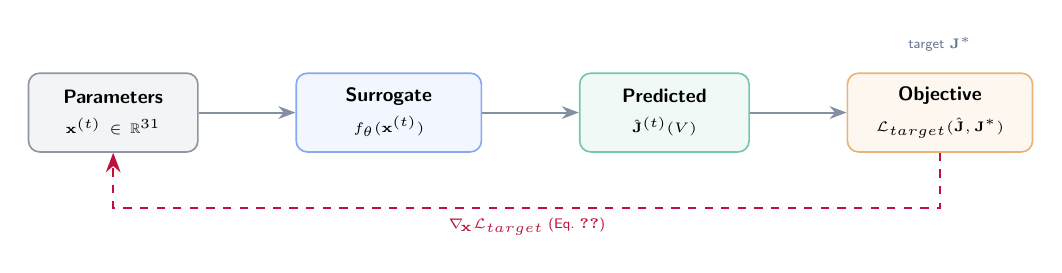
\begin{tikzpicture}[
      >=Stealth,
      every node/.style={font=\sffamily\small},
      block/.style={
        draw=#1!55, fill=#1!6, rounded corners=4pt,
        align=center, line width=0.6pt, inner sep=5pt, minimum height=1cm
      },
      arr/.style={->, line width=0.7pt, color=muted!80},
      garr/.style={->, line width=0.9pt, color=rose, dashed},
    ]
      \node[block=steel, text width=1.8cm] (params) at (0,0) {\textbf{\scriptsize Parameters}\\{\tiny $\mathbf{x}^{(t)} \in \mathbb{R}^{31}$}};
      \node[block=cblue, text width=2.0cm] (surr) at (3.5,0) {\textbf{\scriptsize Surrogate}\\{\tiny $f_\theta(\mathbf{x}^{(t)})$}};
      \node[block=emerald, text width=1.8cm] (jv) at (7,0) {\textbf{\scriptsize Predicted}\\{\tiny $\hat{\mathbf{J}}^{(t)}(V)$}};
      \node[block=amber, text width=2.0cm] (loss) at (10.5,0) {\textbf{\scriptsize Objective}\\{\tiny $\mathcal{L}_{target}(\hat{\mathbf{J}}, \mathbf{J}^*)$}};
      \draw[arr] (params) -- (surr);
      \draw[arr] (surr) -- (jv);
      \draw[arr] (jv) -- (loss);
      \draw[garr] (loss.south) -- ++(0,-0.7)
        -| node[pos=0.25, below, font=\sffamily\tiny, text=rose]
           {$\nabla_{\!\mathbf{x}}\mathcal{L}_{target}$ (Eq.~\ref{eq:inverse})}
        (params.south);
      \node[font=\sffamily\tiny, text=muted, anchor=south] at (10.5,0.65)
        {target $\mathbf{J}^*$};
    \end{tikzpicture}}
    \caption{\textbf{Inverse design loop.} The frozen surrogate $f_\theta$ provides analytic Jacobian gradients for iterative parameter updates toward a target J-V profile $\mathbf{J}^*$. Unlike scalar optimization, curve-level objectives can target specific shape properties (fill factor, knee smoothness, reference matching).}
    \label{fig:inverse_design}
\end{figure}

\paragraph{Sensitivity analysis.}
The Jacobian $\partial \hat{\mathbf{J}}/\partial \mathbf{x}$ also enables systematic sensitivity analysis: which parameters most strongly influence each region of the J-V curve.
This produces physics-interpretable results, e.g., mobilities and lifetimes dominate the knee region, while contact work functions primarily affect $V_{oc}$, that can guide experimental efforts toward the parameters with highest leverage for improving specific aspects of device performance.

%=============================================================================
\section{Conclusion}
\label{sec:conclusion}
%=============================================================================

We presented a physics-constrained dilated convolutional network for J-V curve reconstruction in perovskite solar cells, achieving median $R^2 = 0.9975$ across ${\sim}15$k test devices spanning 31 coupled drift-diffusion parameters with $>$20 orders of magnitude in dynamic range.
The model reconstructs $V_{oc}$ to 0.39~mV median error (below experimental measurement uncertainty) and median MAE of 2.96~A/m$^2$ ($<$0.5\% of typical $J_{sc}$), completing training in ${\sim}10$~min and enabling $>$$10^4\times$ speedup over COMSOL FEM.

Physics knowledge is embedded at every stage of the pipeline: analytically derived drift-diffusion features reduce the 71-candidate input space to 5 features spanning independent physical mechanisms, soft monotonicity, convexity, and curvature penalties enforce qualitative PDE properties on the output, and a modular two-stage design decouples scalar prediction from curve reconstruction.
The architectural choice of bidirectional dilated convolutions is grounded in the physics of J-V responses: thermodynamic equilibria (not temporal sequences) with monotonically decaying spatial correlations that match convolution's local inductive bias, rendering self-attention redundant and consistently harmful on these short sequences.
The differentiable surrogate additionally enables gradient-based inverse design via analytic Jacobians, targeting specific J-V shape properties rather than scalar metrics alone.

Future directions include:
deep-ensemble uncertainty quantification for deployment safety,
Bayesian optimization for closed-loop experimental design,
extension to tandem perovskite/silicon architectures~\cite{zhao2023phd},
end-to-end joint training of both pipeline stages,
and out-of-distribution detection to flag devices outside the training manifold.

%=============================================================================
\appendix
%=============================================================================

\section{Optical Model Details}
\label{app:optical}

Light propagation follows the vectorized transfer-matrix formulation~\cite{zhao2023phd}.
The electric field in layer $n$:
\begin{equation}
E_z(x) = A_n e^{-ik_n(x-L_{n-1})} + B_n e^{ik_n(x-L_{n-1})}
\end{equation}
where $k_n = k_0(n_n - i\kappa_n)$.
Photogeneration rate in the absorber:
\begin{align}
G(x) &= \frac{1}{hc} \int_{\lambda_l}^{\lambda_u} \lambda \, Q(x,\lambda) \, d\lambda \\
Q &= \frac{1}{2} c \varepsilon_0 \alpha n \, |E_z|^2, \quad \alpha = \frac{4\pi\kappa}{\lambda}
\end{align}
A phase-elimination method removes incoherent substrate interference.
$G_{avg} = l_P^{-1}\int_0^{l_P} G(x)\,dx$ enters as one of the 31 inputs.

\section{Full Physics Feature Definitions}
\label{app:features}

\subsection*{Energetics (7)}
\begin{align}
E_g &= \chi_{P}^h - \chi_{P}^e, \quad
V_{bi} = W_{anode} - W_{cathode}, \quad
E_g^{offset} = E_g - V_{bi}
\end{align}

\subsection*{Interface Barriers (9)}
\begin{align}
\Delta E_v^{HP} &= \chi_{HTL}^h - \chi_{P}^h, \quad
\Delta E_c^{PE} = \chi_{ETL}^e - \chi_{P}^e \\
\Phi_{h,ETL} &= \chi_{ETL}^h - \chi_{P}^h, \quad
\Phi_{e,HTL} = \chi_{HTL}^e - \chi_{P}^e
\end{align}

\subsection*{Diffusion Lengths (8)}
\begin{align}
L_n &= \sqrt{\mu_n^P \tau_e k_BT/q}, \quad
L_p = \sqrt{\mu_p^P \tau_h k_BT/q} \\
\eta_{coll,e} &= L_n / l_P, \quad
\eta_{coll,h} = L_p / l_P
\end{align}

\subsection*{$\mu\tau$ Products (4)}
\begin{align}
\mu\tau_e &= \mu_n^P \cdot \tau_e, \quad
\mu\tau_h = \mu_p^P \cdot \tau_h, \quad
\mu\tau_{bal} = \mu\tau_e / \mu\tau_h
\end{align}

\subsection*{Extraction Figures of Merit (6)}
\begin{align}
\mathcal{E}_{bi} &= V_{bi} / l_P, \quad
\Theta_e = \mu_n^P \tau_e V_{bi} / l_P^2 \\
\Theta_h &= \mu_p^P \tau_h V_{bi} / l_P^2, \quad
\Theta_{min} = \min(\Theta_e, \Theta_h)
\end{align}

\subsection*{Series Resistance (5)}
\begin{align}
\sigma_{HTL} &= q \mu_p^{HTL} N_v^{HTL}, \quad
R_s^{HTL} = l_{HTL} / \sigma_{HTL} \\
R_s^{total} &= R_s^{ETL} + R_s^P + R_s^{HTL}
\end{align}

\subsection*{Generation (4)}
\begin{equation}
J_{max} = q \cdot G_{avg} \cdot l_P, \quad
G_{per\,nm} = G_{avg} / l_P
\end{equation}

\subsection*{Recombination (8)}
\begin{equation}
\tau_{eff} = (\tau_e^{-1} + \tau_h^{-1})^{-1}, \quad
V_{oc}^{loss} = -E_g/(k_BT) + \log(R_{SRH})
\end{equation}

\subsection*{Composite Predictors (7)}
\begin{align}
\text{FF}_{pred} &= \log(\Theta_{min}) - \log(R_s^{total}) \\
V_{oc}^{pred} &= E_g + \tfrac{1}{2}(\Phi_{h,ETL} + \Phi_{e,HTL}) - k_BT\log(R_{SRH}) \\
J_{sc}^{pred} &= \log(J_{max}) + \log(\eta_{coll,min}) \\
\text{Quality} &= \log(\Theta_{min}) + \text{SRH}_{str} - \log(R_s^{total})
\end{align}

\section{Full Architecture Ablation}
\label{app:ablation}

Table~\ref{tab:ablation_results} reports the complete ablation spanning 10 configurations $\times$ 3 seeds = 30 runs.
All values are averaged over 3 seeds with $\pm$ indicating seed-to-seed standard deviation.

\begin{table}[h]
\centering
\caption{Architecture ablation (30 runs = 10 configurations $\times$ 3 seeds). All bidirectional conv variants (rows~1--3) achieve $R^2_{med} \geq 0.996$; attention (rows~6--7) and pointwise architectures (row~5) are consistently worse. The champion configuration (row~1, batch~512) achieves the highest median $R^2$ and lowest median MAE.}
\label{tab:ablation_results}
\begin{tabular}{@{}rlcccc@{}}
\toprule
 & \textbf{Configuration} & \textbf{$R^2$ (med.)} & \textbf{MAE$_{med}$} & \textbf{$|V_{oc}|_{med}$} & \textbf{$|I_{sc}|_{med}$} \\
 & & & (A/m$^2$) & (mV) & (A/m$^2$) \\
\midrule
\multicolumn{6}{@{}l}{\emph{Architecture variants (bidir.\ conv, batch 128, 100 ep.)}} \\
1 & \textbf{Conv-Dilated (BS512)} & $\mathbf{.9975{\pm}.0004}$ & $\mathbf{2.96{\pm}.34}$ & $\mathbf{0.39{\pm}.16}$ & $0.36{\pm}.62$ \\
2 & Conv-Dilated & $.9964{\pm}.0007$ & $3.74{\pm}.63$ & $1.04{\pm}.30$ & $0.0{\pm}0.0$ \\
3 & Conv-NoDilation & $.9967{\pm}.0004$ & $3.60{\pm}.36$ & $0.60{\pm}.39$ & $0.66{\pm}.63$ \\
4 & TCN-Dilated (causal) & $.9965{\pm}.0007$ & $3.68{\pm}.67$ & $1.51{\pm}1.68$ & $0.94{\pm}1.63$ \\
5 & Pointwise ($1{\times}1$) & $.9890{\pm}.0004$ & $6.48{\pm}.04$ & $6.11{\pm}1.35$ & $1.31{\pm}1.18$ \\
\midrule
\multicolumn{6}{@{}l}{\emph{Self-attention variants}} \\
6 & Conv-Dilated + Attn & $.9914{\pm}.0006$ & $5.94{\pm}.30$ & $23.7{\pm}39.9$ & $1.59{\pm}.65$ \\
7 & TCN-Dilated + Attn & $.9917{\pm}.0005$ & $5.89{\pm}.61$ & $2.12{\pm}2.53$ & $1.49{\pm}2.59$ \\
\midrule
\multicolumn{6}{@{}l}{\emph{Training \& data variants}} \\
8 & No scalar cond. & $.9966{\pm}.0003$ & $3.63{\pm}.34$ & $0.86{\pm}.33$ & $1.20{\pm}1.51$ \\
9 & 100k data only & $.9948{\pm}.0001$ & $4.57{\pm}.26$ & $0.86{\pm}.58$ & $1.02{\pm}.98$ \\
10 & 200 epochs & $.9965{\pm}.0005$ & $3.69{\pm}.29$ & $1.43{\pm}1.50$ & $0.83{\pm}.75$ \\
\bottomrule
\end{tabular}
\end{table}

\paragraph{Self-attention analysis.}
Adding 4-head self-attention ($d_{model} = 64$) consistently degrades all metrics (rows~6--7 vs.\ rows~2, 4; Figure~\ref{fig:attention_impact}).
The Conv+Attn configuration's extreme $V_{oc}$ instability ($23.7 \pm 39.9$~mV, driven by a single catastrophic seed) further demonstrates that attention introduces harmful optimization landscape pathologies on these short sequences.

\begin{figure}[h]
    \centering
    \includegraphics[width=0.7\textwidth]{dilation_n_attention.png}
    \caption{\textbf{Self-attention consistently degrades performance.}
    Paired comparisons across Conv$\pm$Attn and TCN$\pm$Attn backbones. Adding attention worsens median $R^2$, MAE, $V_{oc}$ error, and $I_{sc}$ error in every case.}
    \label{fig:attention_impact}
\end{figure}

\paragraph{Scalar conditioning.}
Removing upstream scalar conditioning ($V_{oc}^{pred}$, $V_{mpp}^{pred}$; row~8) barely affects median $R^2$ ($0.9966$ vs.\ $0.9967$), confirming that the 31 raw parameters and 5 physics features already encode sufficient information for curve reconstruction.

\paragraph{Data scaling and training duration.}
Using only 100k training samples (row~9) instead of the full ${\sim}120$k degrades $R^2_{med}$ from $0.9967$ to $0.9948$.
Extending training to 200 epochs (row~10) provides no improvement over 100 epochs, indicating convergence within the early-stopping patience window.

\paragraph{Robustness.}
Figure~\ref{fig:architecture_comparison} confirms tight clustering of key metrics across all 30 runs, with all non-attention conv variants achieving median $R^2 > 0.996$ regardless of seed.

\begin{figure}[h]
    \centering
    \includegraphics[width=0.7\textwidth]{fig_architecture_comparison.png}
    \caption{\textbf{Architecture comparison across all 30 runs.} Non-attention conv variants (blue shades) cluster tightly at median $R^2 > 0.996$, while attention variants (red) and pointwise (orange) are clearly separated.}
    \label{fig:architecture_comparison}
\end{figure}

\section{Parameter Distributions}
\label{app:distributions}

Figures~\ref{fig:boxplot_group1}--\ref{fig:boxplot_group4} show the raw parameter distributions grouped by physical type, confirming that the LHS design achieves near-uniform coverage.
Long upper tails in Group~2 (mobilities, permittivities) motivate the $\log_{1p}$ transform applied to material properties during preprocessing (\S\ref{sec:preprocessing}).

\begin{figure}[t]
  \centering
  \includegraphics[width=0.7\textwidth]{group1.png}
  \caption{\textbf{Group~1}: $E_g$, $N_{CV}$, $N_{CC}$. Density-of-states parameters span ${\sim}$3 orders of magnitude. Near-uniform marginals confirm the LHS design.}
  \label{fig:boxplot_group1}
\end{figure}

\begin{figure}[t]
  \centering
  \includegraphics[width=0.7\textwidth]{group2.png}
  \caption{\textbf{Group~2}: $\mu_e$, $\mu_h$, $\varepsilon$, $A$. Long upper tails from log-uniform sampling, motivating the $\log_{1p}$ transform in preprocessing.}
  \label{fig:boxplot_group2}
\end{figure}

\begin{figure}[t]
  \centering
  \includegraphics[width=0.7\textwidth]{group3.png}
  \caption{\textbf{Group~3}: $C_n$, $C_p$, $N_t$, $E_t$, $n_D$, $n_A$. Recombination and doping parameters.}
  \label{fig:boxplot_group3}
\end{figure}

\begin{figure}[t]
  \centering
  \includegraphics[width=0.7\textwidth]{group4.png}
  \caption{\textbf{Group~4}: Thicknesses, $T$, $S_{n,p}$, $R_s$, $R_{sh}$, $G$, light intensity.}
  \label{fig:boxplot_group4}
\end{figure}

\section*{Code and Data Availability}

Training and inference code is available at \url{https://github.com/memo-ozdincer/perovskite-jv-surrogate}.
Pre-trained model checkpoints and preprocessing artifacts are hosted on HuggingFace at \url{https://huggingface.co/memo-ozdincer/perovskite-jv-surrogate}.
The COMSOL simulation dataset (${\sim}150$k devices, 31 parameters, 45-point J-V curves) is available at \url{https://huggingface.co/datasets/memo-ozdincer/perovskite-jv-comsol-150k}.

%=============================================================================
\begin{thebibliography}{99}

\bibitem{zhao2025ae}
X. Zhao, C. Huang, E. Birgersson, N. Suprun, H.Q. Tan, Y. Zhang, Y. Jiang, C. Shou, J. Sun, J. Peng, and H. Xue,
``Accelerating device characterization in perovskite solar cells via neural network approach,''
\textit{Applied Energy}, 392:125922, 2025.

\bibitem{zhao2023phd}
X. Zhao,
``Mathematical Modeling of Two-terminal Perovskite-Based Thin-film Tandem Solar Cells,''
Ph.D. thesis, National University of Singapore, 2023.

\bibitem{fritsch1980monotone}
F.N. Fritsch and R.E. Carlson,
``Monotone Piecewise Cubic Interpolation,''
\textit{SIAM J. Numer. Anal.}, 17(2):238--246, 1980.

\bibitem{kendall2018multi}
A. Kendall, Y. Gal, and R. Cipolla,
``Multi-Task Learning Using Uncertainty to Weigh Losses,''
\textit{CVPR}, 2018.

\bibitem{burden2008bayesian}
F. Burden and D. Winkler,
``Bayesian regularization of neural networks,''
in \textit{Methods in Molecular Biology}, Humana Press, pp. 23--42, 2008.

\bibitem{feng2024bandgap}
S. Feng et al.,
``Prediction of Organic-Inorganic Hybrid Perovskite Band Gap by Multiple ML Algorithms,''
\textit{Molecules}, 29:499, 2024.

\bibitem{talapatra2021formability}
A. Talapatra et al.,
``A ML approach for formability and stability of perovskite oxides,''
\textit{Chem. Mater.}, 33:845--858, 2021.

\bibitem{zhang2020lattice}
Y. Zhang and X. Xu,
``Machine learning lattice constants for cubic perovskite compounds,''
\textit{ChemistrySelect}, 5:9999--10009, 2020.

\bibitem{hu2022ml}
Y. Hu et al.,
``Machine-learning modeling for ultra-stable high-efficiency perovskite solar cells,''
\textit{Adv. Energy Mater.}, 12, 2022.

\bibitem{oboh2024nn}
I.O. Oboh et al.,
``Explainable ML for predicting band gaps of ABX3 perovskites,''
\textit{Mater. Sci. Semicond. Process.}, 161:107427, 2023.

\bibitem{courtier2019transport}
N.E. Courtier et al.,
``How transport layer properties affect perovskite solar cell performance,''
\textit{Energy \& Environ. Sci.}, 12:396--409, 2019.

\bibitem{toprak2025jv}
A. Toprak,
``High-accuracy ML approach for predicting J-V characteristics of perovskite solar cells,''
\textit{Scientific Reports}, 15:41304, 2025.

\bibitem{zbinden2026ae}
O. Zbinden, E.L. Comi, E. Knapp, and W. Tress,
``Autoencoder for parameter estimation and J-V simulation of perovskite solar cells,''
\textit{npj Computational Materials}, 12:7, 2026.

\end{thebibliography}

\end{document}
